\documentclass{VUMIFPSbakalaurinis}
\usepackage{float}
\usepackage{hyperref}
\usepackage{algorithmicx}
\usepackage{algorithm}
\usepackage{algpseudocode}
\usepackage{amsfonts}
\usepackage{amsmath}
\usepackage{bm}
\usepackage{caption}
\usepackage{color}
\usepackage{graphicx}
\usepackage{listings}
\usepackage{subcaption}
\usepackage{wrapfig}
\usepackage{biblatex}
\usepackage{microtype}

% Titulinio aprašas
\university{Vilniaus universitetas}
\faculty{Matematikos ir informatikos fakultetas}
\institute{Informatikos institutas}  % Užkomentavus šią eilutę - institutas neįtraukiamas į titulinį
\department{Programų sistemų bakalauro studijų programa}
\papertype{Bakalauro baigiamasis darbas}
\title{„Mono2Micro“ tikslumo ir tinkamumo vertinimas monolitinių sistemų migravime}
\titleineng{Evaluating the Accuracy and Usability of Mono2Micro in Microservice Migration}
\author{Audrius Kumpis}
% \secondauthor{Vardonis Pavardonis}   % Pridėti antrą autorių
\supervisor{lekt. Vasilij Savin}
\reviewer{doc. dr. Audronė Lupeikienė}
\addsignatureplaces{} % prideda parašų vietas tituliniame puslapyje
\date{Vilnius – \the\year}

\bibliography{bibliografija}

\begin{document}
\maketitle

\sectionnonumnocontent{Santrauka}
Sparčiai diegiant mikroservisų architektūrą reikia veiksmingų priemonių, kurios padėtų pereiti nuo monolitinių sistemų. IBM „Mono2Micro“ yra vienas iš įrankių, skirtų šiam migravimo procesui automatizuoti ir palengvinti. Tačiau reikia sistemingai įvertinti jos patikimumą ir pagrįstumą, kad būtų užtikrintas jos veiksmingumas realiomis sąlygomis. Šio darbo tikslas - atlikti išsamų „Mono2Micro“ vertinimą naudojant patikimų ir kiekybiškai įvertinamų rodiklių rinkinį. Vertinimas sutelktas į „Rekomendacijų tikslumą“, „Sėkmingo įgyvendinimo lygį“ ir „Įgyvendinimo sėkmės lygį“ kriterijus. Nors šio darbo rezultatai rodo didelį „Mono2Micro“ patikimumą ir pagrįstumą bandomuose scenarijuose, jie taip pat pabrėžia, kad kartu su automatizuotomis priemonėmis reikia žmogiškosios kompetencijos ir strateginio numatymo. Ateityje būtų galima išbandyti „Mono2Micro“ su įvairesnėmis monolitinėmis taikomosiomis programomis ir palyginti jo veikimą su kitais migravimo įrankiais. Šis tyrimas prisideda prie „Mono2Micro“ veiksmingumo supratimo ir pateikia įžvalgų, kuriomis būtų galima vadovautis taikant šią priemonę ateityje.
\raktiniaizodziai{„Mono2Micro“, Mikroservisų architektūra, Monolitinė architektūra, Programų sistemų pertvarkymas, Programų sistemų patikimumas, Programų sistemų pagrįstumas}

\sectionnonumnocontent{Summary}
The rapid deployment of microservices architectures requires effective tools to move away from monolithic systems. IBM's Mono2Micro is one such tool designed to automate and facilitate this migration process. However, its reliability and validity need to be systematically evaluated to ensure its effectiveness in real-life conditions. The aim of this work is to carry out a comprehensive evaluation of Mono2Micro using a set of reliable and quantifiable indicators. The evaluation focuses on the criteria of "Accuracy of recommendations", "Level of successful implementation" and "Level of implementation success". While the results of this work show the high reliability and validity of Mono2Micro in the scenarios tested, they also highlight the need for human expertise and strategic foresight in combination with automated tools. Future work could test Mono2Micro with a wider range of monolithic applications and compare its performance with other migration tools. This study contributes to the understanding of the effectiveness of Mono2Micro and provides insights to guide future applications of the tool.
\keywords{Mono2Micro, Microservices, Monolithic Systems, Software Refactoring, Software Reliability, Software Validity}

\tableofcontents

\sectionnonum{Įvadas}
Kai komanda pradeda kurti programą, monolitas įprastai yra numatytas pasirinkimas. Tai yra viena pagrindinių priežasčių, kodėl egzistuoja itin daug monolitinių sistemų. Monolitas turi savo duomenų bazę, savo funkcionalumo įgyvendinimą ir tai yra vientisa programa. Jis yra lengvai suprogramuojamas ir su palyginamai nedideliu darbo indėliu, galima greitai sukurti bei diegti veikiančią sistemą. Tačiau tokią architektūrą yra labai sunku plėtoti bei palaikyti. Kuo daugiau  tokia sistema yra plėtojama, tuo daugiau ji didėja, daugėja kodo bei priklausomybių nuo kitų sistemų. Anot S. Newman, mikroservisų architektūros specialisto, tuomet diegimai tampa ilgi ir itin reti. Testavimas būna sudėtingas, nes negalima atlikti izoliuoto atskirų sistemos modulių testavimo \cite{New19}. Kad ši problema būtų išspręsta, paprastai monolitinės sistemos yra skaidomos į mikroservisus \cite{DK}.

Mikroservisai – tai atskiri, nedideli servisai, kurie atsakingi už tam tikras specifines užduotis. Jie yra implementuoti kaip atskiros programos, o komunikacija tarp jų įprastai yra vykdoma per pranešimų siuntimo (angl. messaging) technologijas arba per REST API. Kiekvienas mikroservisas turi savo duomenų bazę, savo diegimo strategijas bei testavimo aplinką. Mikroservisų architektūra suteikia daug privalumų \cite{FBZ+19}, pavyzdžiui:
\begin{itemize}
    \item Pagreitinami sistemos diegimai.
    \item Pagerinamas sistemos plečiamumas.
    \item Nėra priklausomybės nuo pasirinktų technologijų.
    \item Prie sistemos implementacijos gali dirbti didesnis komandų skaičius.
\end{itemize}

Nors mikroservisai išsprendžia daug problemų, tai nėra paprastas sprendimas. Kadangi migravimas į mikroservisų architektūrą yra pilnai techninė užduotis, privaloma gauti projekto vadovo ir/ar projekto savininko sutikimą, kad migracijai būtų skiriami resursai bei lėšos. Viena iš sunkesnių migracijos dalių yra mikroservisų projektavimas. Yra daugybė būdų, kaip galima išskaidyti monolitinę sistemą į mažesnius servisus \cite{FBZ+19}, taigi iš anksto apgalvoti, kokia strategija bus taikoma yra svarbu ir laiko, ir resursų atžvilgiu. Kad migracija iš monolitinės architektūros į mikroservisų būtų sklandi, reikia gerai žinoti, kokius darbus ir kokia tvarka būtina atlikti. Jau egzistuoja keletas migravimo atlikimo strategijų \cite{Wal22,MQO18,KXL+20}, su kuriomis susipažinus yra lengviau suplanuoti reikiamus darbus. Šiame darbe bus aptartos šios strategijos:
\begin{itemize}
    \item Migravimas skaidant domenus.
    \item Migravimas pasinaudojant dirbtiniu intelektu paremtą įrankį „Mono2Micro“.
\end{itemize}

\sectionnonum{Darbo tikslas ir uždaviniai}
Darbo tikslas: įvertinti „Mono2Micro“ techninės galimybės bei pateikti rekomendacijas būsimiems įrankio naudotojams. Taip pat šio tyrimo tikslas yra prisidėti prie augančio žinių apie mikroservisų architektūrą kiekio ir pateikti praktinių įžvalgų informacinių technologijų specialistams, dalyvaujantiems programinės įrangos modernizavimo iniciatyvose.

Šio darbo uždaviniai bus trys: darbe bus atlikta problemos analizė, bus atliktas eksperimentas, kurio tikslas bus įvertinti įrankio savybes, ir pagal eksperimento rezultatus atlikti įrankio vertinimą. Tyrimo tikslams pasiekti bus atliekamos kelios užduotys. Pirma, bus analizuojama monolitinė programa, siekiant nustatyti jos pagrindines funkcijas ir priklausomybes. Antra, bus naudojamas įrankis „Mono2Micro“, kad monolitinė programa būtų migruota į mikroservisų architektūrą, remiantis domenais grindžiamo projektavimo principais. Trečia, bus atliktas eksperimentas, kurio siekis bus įvertinti įrankio kokybiškumą atsižvelgiant į gerąsias mikroservisų architektūros praktikas. Atlikus šias užduotis bus padaryta išvada, ar „Mono2Micro“ yra tinkamas įrankis monolitinių sistemų migravimo į mikroservisų architektūrą užduočiai.

\section{Dekomponavimas skaidant domenus}
Pirmiausia bus aptarta vieną iš populiariausių migravimo strategijų – skaidymas pagal domenus \cite{Wal22}. Šią strategiją verta naudoti tuomet, kai verslo panaudos sritys yra aiškiai išskirtos. Dažnai  ši sąlyga būna neįgyvendinta, todėl yra itin svarbu į monolito pertvarkymo procesą įtraukti verslo atstovus, analitikus bei kitus techninius sistemos atstovus, kurie gerai supranta perdaromos sistemos funkcionalumą esančiame įgyvendinime.

\subsection{Strategijos aprašymas}
Dekomponavimas skaidant domenus (angl. domain-driven refactoring) yra viena iš populiariausių migravimo strategijų. Ją geriausia naudoti tuomet, kai monolitas buvo kurtas laikantis domenais paremtu kūrimu (angl. domain-driven development). Tačiau ne visada būna taip, jog monolitas yra jau iš karto paruoštas migravimui. Pirmas ir svarbiausias žingsnis yra esminių domenų identifikavimas \cite{LZ22}. Kad esminių domenų identifikavimas būtų atliktas sėkmingai, privaloma įtraukti visus suinteresuotuosius asmenis minėtus anksčiau. Kad nauja architektūra tinkamai atliktų užduotis, privaloma investuoti laiko į monolito servisų sėkmingą migravimą į atskirus servisus. 

Šios problemos sprendimas buvo pristatytas 2011 metais, o mikroservisų idėja buvo pristatyta 2005 metais. Sprendimo idėja yra paprasta: kai naujo domeno funkcionalumas yra įgyvendintas mikroservise ir jau yra paruoštas naudojimui, sistema perima naujojo mikroserviso funkcionalumą ir nebenaudoja jo iš senosios sistemos. Tai yra daroma su kiekvienu esminiu, atrinktu domenu. Tokiu būdu, monolitas yra „smaugiamas“ tol, kol jame nebebus nei vieno naudojamo domeno. Iš to ir seka šios taktikos pavadinimas – „Smaugiko šablonas“ \cite{Beh18}. Šis šablonas yra taikomas beveik visuomet, kai yra naudojamas dekomponavimo pagal domenus strategija.

\subsection{Strategijos pritaikymas}
Šiame pavyzdyje naudojama fiktyvi paskolų išdavimo sistema. Šioje sistemoje yra naudojami 5 esminiai domenai: autentikacijos, paskolos dydžio skaičiuoklė, išmokėjimo mechanizmas, kreditingumo skaičiuoklė, transakcijų gavimo mechanizmas. Visi šie domenai veikia darnoje ir yra priklausomi vienas nuo kito. Jų veikimas pavaizduotas šioje diagramoje:
\begin{figure}[H]
    \centering
    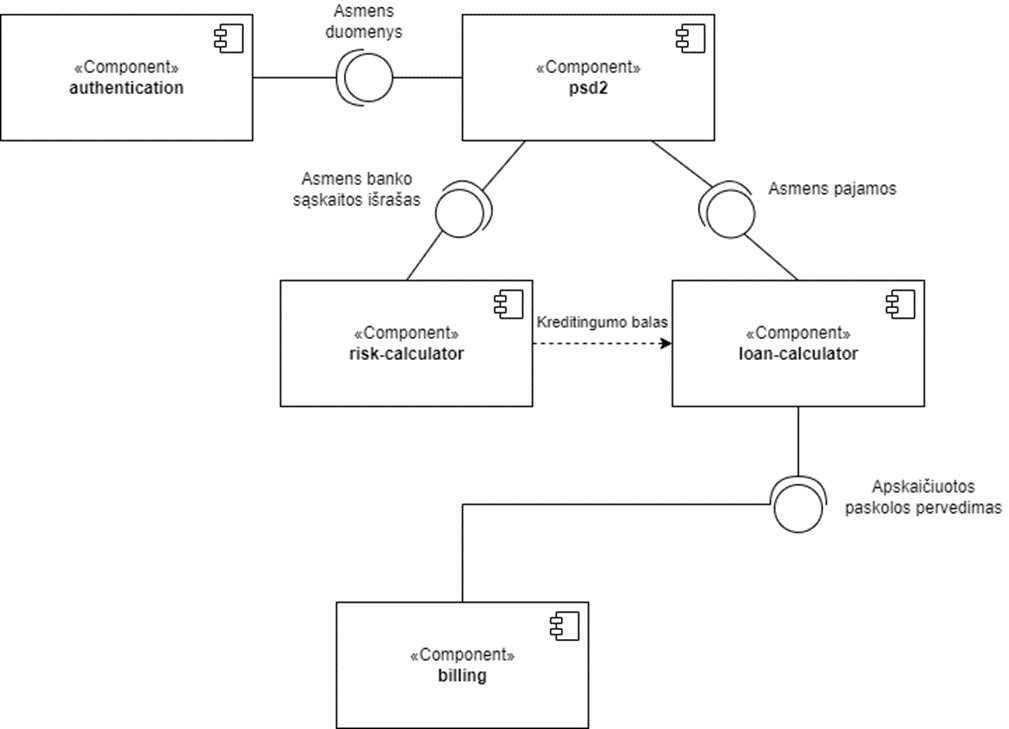
\includegraphics[scale=0.9]{img/komponentu-diagrama.png}
    \caption{Pavyzdinio monolito komponentų diagrama}
    \label{img:komponentu-diagrama}
\end{figure}

Visi šie domenai – komponentai – priklauso vienas nuo kito. Jei bent vienas neveikia, arba veiks klaidingai, tai atneš nenumatytų nuostolių verslui. Pasinaudojant „smaugiko“ šablonu, iteratyviai kiekvienam išskirtam domenui, yra sukuriamas mikroservisas. Kūrimo metu yra privaloma užtikrinti, jog bendras sistemos veikimas nėra sugadinamas, jog sistema vis dar veikia korektiškai. Kad tai būtų užtikrinta, privaloma kuo anksčiau sukonfigūruoti pastovaus diegimo/pastovaus testavimo liniją. (angl. CI/CD pipeline)  Supaprastintą šablono panaudojimą galima pamatyti \ref{img:smaugiko-sablonas} pav.

\begin{figure}[H]
    \centering
    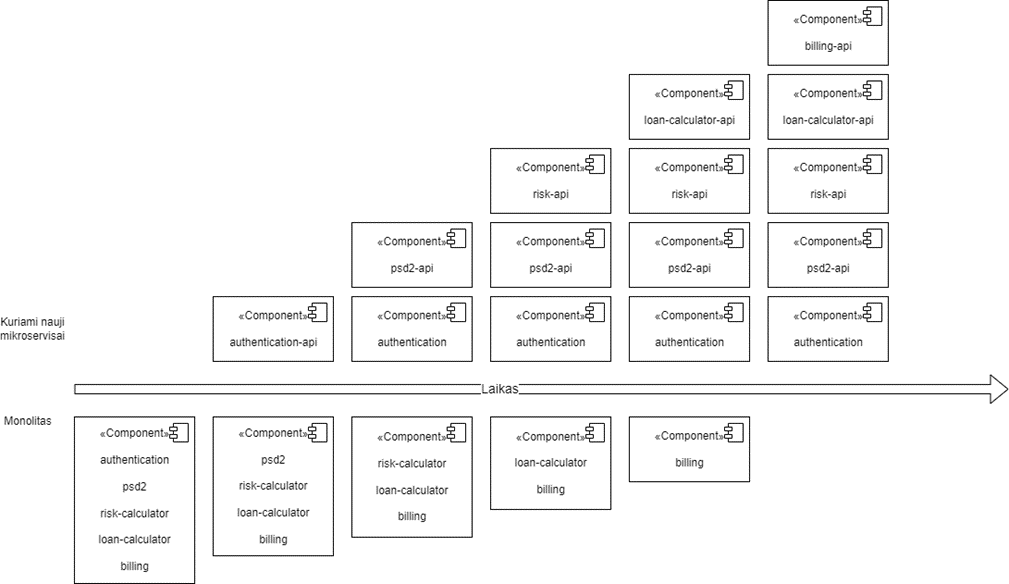
\includegraphics{img/smaugiko-sablonas.png}
    \caption{„Smaugiko“ šablono įgyvendinimas}
    \label{img:smaugiko-sablonas}
\end{figure}

Naujai sukurtiems mikroservisams yra būtina kuo anksčiau priskirti atsakingas komandas. Šios komandos bus atsakingos už tolimesnius mikroservisų darbus, priežiūrą, keitimus, bei teisingos integracijos su dar laikinai naudojamu monolitu užtikrinimą. Taigi prieš visą migraciją privaloma įsivertinti, ar programavimo komandoje pakanka resursų priskirti žmones specifiniams mikroservisams.

Iš karto gali kilti klausimas: kaip atsirinkti, ką pirmiausia reikia iškelti į naują mikroservisą? Jei šis šablonas yra taikomas pirmą kartą programavimo komandoje, saugiausias variantas būtų pradėti nuo mažiausiai reikšmingo ir/ar mažiausio pagal dydį komponento. Tokiu būdu, komanda įgautų daugiau patirties darbui labiau svarbiems komponentams. Be šito, kiti galimi kandidatai yra \cite{Beh18}:
\begin{itemize}
    \item Komponentai, kurie yra labiausiai užbaigti. Jie turi didžiausią padengimo testais procentą, mažiausiai neužbaigtų techninių darbų. Programavimo komanda tuomet jaustųsi saugiausiai migruodama šį komponentą.
    
    \item Komponentai, kurie tikėtina, jog plėsis labiausiai. Iškėlus juos į mikroservisus pirmiausia, tikėtina, jog reikės perkelti mažiau kodo, nei tą darbą atliekant vėliau.
    
    \item Komponentai, kurie dažniausiai kinta dėl besikeičiančių verslo reikalavimų. Tai užtikrintų, jog atliekant verslo reikalaujamus pakeitimus, nereiktų diegti viso monolito, užtektų diegti tik naują mikroservisą.\\
\end{itemize}

\subsection{Įvertinimas}
Taigi, šią migravimo strategiją rekomenduojama naudoti tuomet, kai yra aiškiai apibrėžti domenai, arba jei yra galimybė įtraukti verslo atstovus aiškių esminių domenų identifikavimui. Tačiau ši strategija nėra tinkama visiems atvejams. Jos nerekomenduojama naudoti tuomet, kai monolitas yra dar itin mažos apimties ir neturi aiškiai apibrėžtų esminių domenų. Priešingu atveju, gali būti brangu sumodeliuoti, kurti bei prižiūrėti naujai sukurtus mikroservisus. Naudojantis šia strategija, atliekamo pertvarkymo darbo laikas tiesiogiai priklauso nuo esamo monolito dydžio. Kuo didesnis monolitas, tuo ilgiau truks jį išskaidyti. Sunkiausia dalis visgi lieka esminių domenų identifikavimas. Taip pat, jei esamame monolite yra didelis kodo padengimas funkciniais testais, tai gali padėti užtikrinti, jog migravimas bus sėkmingas ir reikės atlikti mažiau pilno testavimo rankiniu būdu.

\section{Dekomponavimas naudojant „Mono2Micro”}
Per pastaruosius metus šis metodas pritraukė daug dėmesio. Jo pagalba galima palengvintu būdu atskirti esminius domenus bei juos iškelti į naujus mikroservisus. Naudojantis šiuo įrankiu klaidų tikimybė yra tikėtinai mažesnė, monolito migravimas tampa greitesnis už tradicinius metodus bei turi galimybę paruošti naujus mikroservisus būti naudojamiems debesijoje (angl. cloud computing). Šio darbo rašymo metu, įrankis sėkmingai atlieka migravimo užduotis tik su Java kalba parašytoms programoms, tačiau ateityje yra numatoma apjungti ir kito tipo programas \cite{KXL+20}.

\subsection{Strategijos aprašymas}
„Mono2Micro“ (toliau įrankis) yra dirbtinio intelekto pagalba sukurtas įrankių rinkinys, kuris padeda pertvarkyti esamą seną sistemą į mikroservisų architektūrą. Įrankis leidžia vartotojui pasirinkti norimus panaudos atvejus ir programos veikimo metu juos priskirti esančioms klasėms, servisams. Įrankis taip pat atlieka statinę programos analizę ir surenka programos struktūrinę informaciją bei priklausomybes. Šią informaciją tuomet analizuoja dirbtinio intelekto variklis ir sukuria programos padalinius (angl. partitions) pagal verslo panaudos atvejų ir priklausomybių panašumą bei panaudojimą. Sugeneruoti padaliniai yra potencialūs kandidatai naujam mikroservisui. Vartotojas gali peržiūrėti šiuos padalinius, juos redaguoti ar kitaip grupuoti, kad būtų gautas kuo tikslesnis norimas mikroservisas \cite{KXK+21}. Taip pat, kartu su verslo panaudos atvejais, įrankis sugeneruoja natūraliai panašius padalinius. Jie skiriasi tuo, jog nėra analizuojama duomenų priklausomybė. Taip galima supaprastinti duomenų priklausomybes tarp sugeneruotų padalinių.

\begin{figure}[H]
    \centering
    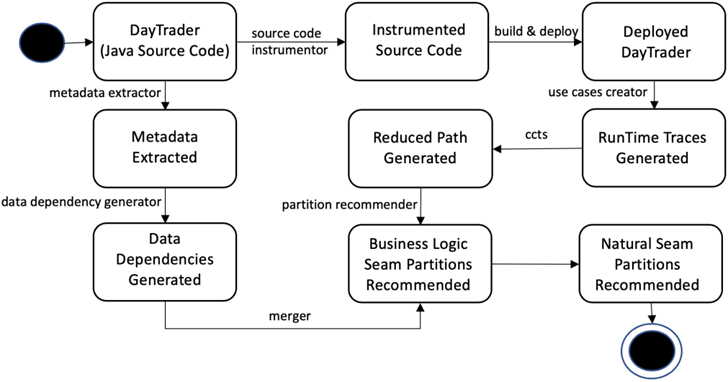
\includegraphics{img/mono-2-micro-veikimas.png}
    \caption{Verslo panaudos atvejų ir natūraliai panašių padalinių generavimas naudojantis „Mono2Micro“ įrankiu \cite{KXL+20}.}
    \label{img:mono-2-micro}
\end{figure}

Kad įrankis sugeneruotų tikslius panaudos atvejus, programa, kurią norima pertvarkyti yra startuojama. Kai ji pradeda veikti, per vartotojo sąsają būtina atlikti visus panaudos atvejus. Jei kuris nors atvejis bus praleistas, įrankis ieškos daugiau panaudos atvejų funkciniuose testuose. Visa ši informacija yra surenkama į orientuotą grafą $(V, E)$. kur $V$ yra klasės, $E$ yra veikimo metu nustatyti metodų kvietimo sąryšiai tarp klasių \cite{KXL+20}. Sugeneruoto grafo pavyzdys parodomas \ref{img:mono-micro-grafas} pav.

\begin{figure}[H]
    \centering
    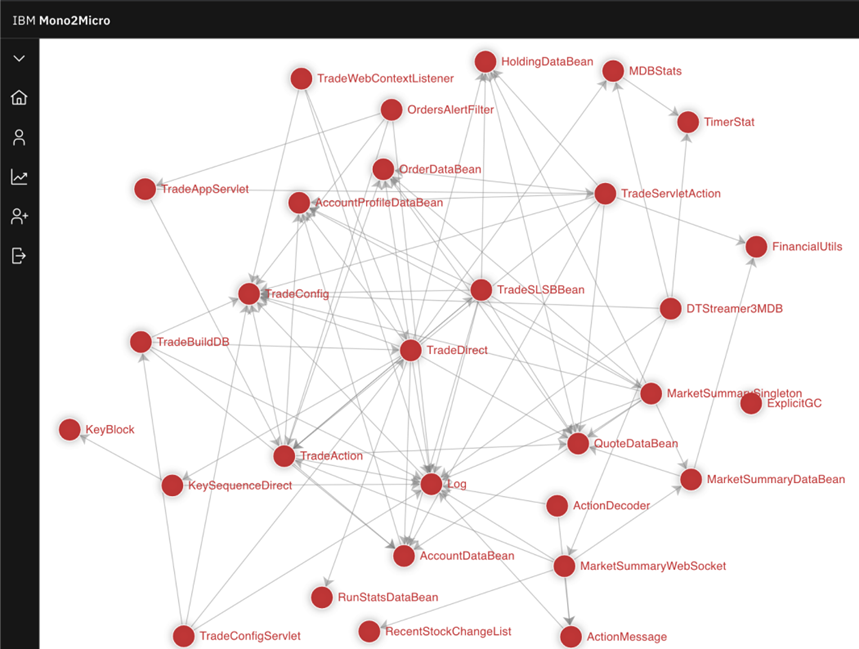
\includegraphics{img/mono-micro-grafas.png}
    \caption{Veikimo metu sugeneruotas orientuotas grafas $(V, E)$, parodantis dinaminius sąryšius tarp klasių \cite{KXL+20}.}
    \label{img:mono-micro-grafas}
\end{figure}

Surinkus visą reikiamą informaciją apie klases ir jų ryšius, įrankis gali pasinaudoti šiais duomenimis bei sugeneruotu kvietimo konteksto medžiu (angl. calling-context tree), kad sukurtų padalinių rekomendacijas. Turint norimą padalinių skaičių $k$ ir klasių aibę $C = {c_{1}, c_{2}, ..., c_{n}}$ galima sugrupuoti klases pasinaudojant šia panašumo formule \cite{KXL+20}.

\begin{equation}\label{eq:panasumo-formule}
    Sim_{i,j} = \frac{\sum_{m=o}^{n_{i}}\sum_{n=0}^{n_{j}}S(c_{im},C_{jn})}{\left| C_{i} \right|\left| C_{j} \right|}
\end{equation}

Panašumo dydis yra apskaičiuojamas remiantis tiesioginiais ir netiesioginiais kvietimų ryšiais tarp klasių $c_{i}$ ir $c_{j}$. Tiesioginio kvietimo ryšys egzistuoja tik tuomet, kai ryšys tarp klasių $c_{i}$ ir $c_{j}$ kvietimo konteksto medyje egzistuoja briauna $(c_{i}, c_{j})$. Netiesioginio kvietimo ryšys tarp klasių $c_{i}$ ir $c_{j}$ egzistuoja tik tuomet, jei konteksto kvietimo medyje egzistuoja kelias $(c_{i}, c_{2}, ..., c_{p}, c_{j}), p > 1$.

Kai yra sugeneruojami padaliniai pagal panaudos atvejų panašumą, įrankis juos sujungia pagal natūralų panašumą. Jei klasės $c_{i}$ ir $c_{j}$ turi ryšių, jos yra priskiriamos vienam padaliniui. Tokiu būdu pereinama per visas visų padalinių klases ir gaunamas optimalus natūraliai panašių padalinių skaičius.

\subsection{Strategijos pritaikymas}
Šiai strategijai išbandyti buvo naudojama populiari „IBM“ sukurta etaloninė programa „DayTrader“ \cite{IBM15}. Tai yra elektroninė akcijų pirkimo ir pardavimo programa. Ji leidžia vartotojui prisijungti, peržiūrėti savo profilį, peržiūrėti esamas akcijas, jų kainas bei kainų istoriją, pirkti bei parduoti akcijas. Joje yra 112 klasių ir 964 metodų. Kodo padengimas funkciniais testais: padengta  66 \% klasių, 44 \% metodų. Pasinaudojus įrankiu ir nurodžius padalinių skaičių $k = 7$ gauname rekomenduojamus 3 padalinius $p_{1}, p_{2}, p_{3}$.

\begin{figure}[H]
    \centering
    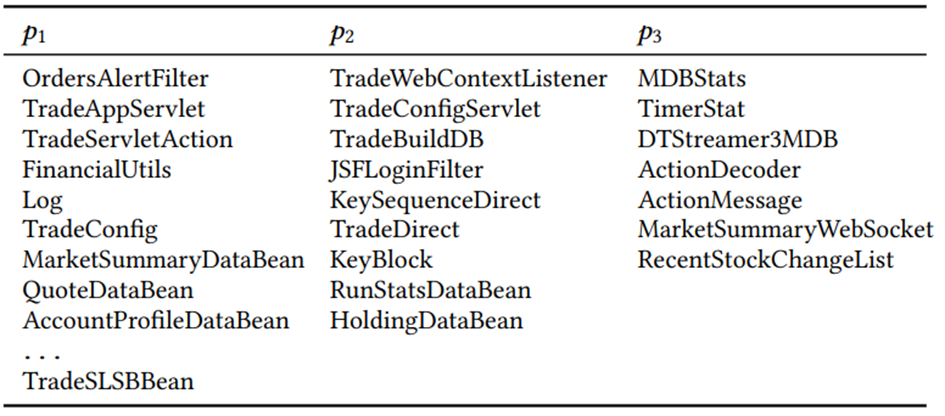
\includegraphics{img/mono-micro-padaliniai.png}
    \caption{Sugeneruoti padaliniai „DayTrader“ programai, kai $k = 7$, \cite{KXK+21}}
    \label{img:mono-micro-padaliniai}
\end{figure}

Padalinyje $p_{1}$ yra priskiriamos klasės, susijusios su akcijų pirkimo ir pardavimo funkcionalumu, $p_{2}$ yra priskiriamos klasės, susijusios su duomenų bazės operacijomis, o $p_{3}$ yra priskiriamos klasės susijusios su įvairių pranešimų siuntimu. Šie padaliniai buvo suskirstyti pagal atliekamas programines funkcijas ir jie nėra glaudžiai susiję su verslo moduliais pasinaudojant įrankio padalinių sujungėju. Parodžius šiuos rezultatus programinės įrangos architektams, kurie yra susipažinę su šia programa, jie patvirtino, jog šie „Mono2Micro“ sugeneruoti mikroservisų patarimai yra logiški ir prasmingi \cite{KXL+20}.\\

\subsection{Įvertinimas}
„Mono2Micro“ tinka sugeneruoti esamo Java EE monolito pertvarkymo rekomendacijoms. Šis įrankis yra lankstus, suteikiantis daug patarimų ir rekomendacijų, ir parodė, jog veikia gerai su vidutinio dydžio Java Spring programomis \cite{San21}. Tačiau įrankis daugiau dėmesio skiria sugrupuoti esamas klases pagal jų techninį funkcionalumą, o ne pagal verslo panaudos atvejus, kas yra įprastas mikroservisų tikslas. Taip pat pastebėtina, jog šis įrankis gali būti naudojamas ne tik monolito paruošimui mikroservisų architektūrai, bet ir patikrinimui, ar monolitą tikrai verta skaldyti į atskirus mikroservisus. Jei gaunamas rekomenduotinų padalinių skaičius yra nedidelis (pvz., 2), tai verta pamąstyti, ar apsimoka skirti laiko ir resursų šiam sudėtingam darbui. Nors šis įrankis šiuo metu veikia tik su Java programomis, tikėtina, jog jis ateityje palengvins ir kitokio tipo programų pertvarkymą.

\section{„Mono2Micro“ praktinis pritaikymas bei kokybės vertinimas}
Šiame darbe bus atliekamas monolitinės sistemos „E Shop“ migravimas naudojantis „Mono2Micro“ migravimo įrankiu. Migravimo metu bus vertinamas šio įrankio patikimumas, ekseprimento rezultatų pagrįstumas bei panaudojamumas. Šio eksperimento rezultatai priklauso nuo aplinkos, kurioje jie yra vykdomi. Tikėtinas šių eksperimentų rezultatas yra aukštas įrankio patikimumas bei panaudojamumas. Taip pat pastabos, patarimai ir įžvalgos, kaip šis įrankis gali būti pagerintas ar kaip juo naudotis, kad būtų pasiektas geriausias migravimo rezultatas.

Atlikus šiuos eksperimentus bus atlikta monolitinės sistemos migracija į „Mono2Micro“ parekomenduotus mikroservisus. Tada bus patikrinama, ar ši nauja sistema vis dar atlieka jai būdingus panaudos atvejus, bus lyginamas jos ir monolitinės sistemos našumas.

% Gal reik kitur idet? Ar reik isvis?
\subsection{Problemos formuluotė}
Monolitinių programų migravimas iš monolitinės architektūros į mikroservisų architektūrą yra sudėtingas ir dažnai sudėtingas procesas, kuris tampa vis aktualesnis šiuolaikiniame technologijų kraštovaizdyje. Šiam procesui padėti sukurta įvairių priemonių, viena iš jų - IBM „Mono2Micro“. Nors ši priemonė suteikia daug žadančių galimybių, išsamus jos patikimumo ir kokybės vertinimas nėra pakankamai atliktas. Todėl trūksta žinių apie tikrąjį „Mono2Micro“ veiksmingumą, ypač apie jo gebėjimą nuolat teikti tikslias rekomendacijas, sėkmingo vykdymo rodiklį, rekomenduojamų mikroservisų sėkmingo įdiegimo galimybes ir bendrą patogumą naudotojo požiūriu. Programinės įrangos kūrimo kontekste, kur patikimos priemonės gali turėti didelę įtaką produktyvumui ir galutinio produkto kokybei, šis klausimas yra didelė problema. Todėl sistemingas „Mono2Micro“ patikimumo ir kokybės įvertinimas yra būtinas ir vertingas darbas, kuris padėtų informuoti apie praktinį jo taikymą ir tolesnį vystymą.

\subsection{Įrankių vertinimo metodikos}
Programų sistemų inžinerijoje vertinant pagalbines programinės įrangos priemones, reikia taikyti išsamų ir sistemingą metodą, kad būtų galima įvertinti jų patikimumą, veiksmingumą ir bendrą kokybę. Pagrindiniai šio vertinimo proceso aspektai yra funkcinis testavimas, tinkamumo naudoti testavimas, našumo testavimas, saugumo testavimas ir integravimo galimybės \cite{NVS+19}. Funkciniu testavimu įvertinama, ar priemonė tinkamai atlieka numatytas užduotis įvairiomis sąlygomis. Naudojamumo testais vertinama priemonės naudotojo sąsaja, jos naudojimo paprastumas, funkcijų ir pranešimų apie klaidas suprantamumas. Atliekant našumo testavimą analizuojamas priemonės atsako laikas ir stabilumas esant skirtingoms darbo apkrovoms ir streso sąlygoms. Saugumo testavimas yra labai svarbus aspektas, kurio metu tiriamos galimos priemonės pažeidžiamosios vietos, kuriomis galėtų pasinaudoti įsilaužėliai. Be to, labai svarbus vertinimo kriterijus yra priemonės gebėjimas sklandžiai integruotis su kita programine įranga ir sistemomis. Dokumentacijos kokybė, atnaujinimų dažnumas, galimybė gauti pagalbą ir realių naudotojų atsiliepimai taip pat labai prisideda prie išsamaus šių pagalbinės programinės įrangos priemonių vertinimo. Toks daugialypis vertinimo metodas užtikrina priemonės tvirtumą, patikimumą ir tinkamumą teikti numatytą naudą.

„Mono2Micro“ kontekste, visi šie punktai yra taikytini, išskyrus našumo, saugumo testavimas ir integravimo sugebėjimas. Našumo testavimas nebus testuojamas, nes „Mono2Micro“ nėra tokia programa, kuri privalo pasižymėti dideliu našumu. Saugumo testavimas taip pat nėra aktualus, nes šis įrankis nėra eksponuojamas internete, taigi nėra pažeidžiamas įvairioms kibernetinėms atakoms. Integravimosi sugebėjimo testavimas taip pat nėra aktualus, nes šis įrankis yra naudojamas kaip atskira programa ir nesiintegruoja su jokiomis kitomis sistemomis.

\subsection{Pasiruošimas vertinimui}
% nežinau, ar verta šitai paminėti
„Mono2Micro“ yra mokamas IBM įrankis, skirtas atlikti migravimą IBM WebSphere Open Liberty serveryje, tačiau šis įrankis pateikia mikroservisų rekomendacijas nepriklausomai nuo vykdomosios aplinkos. Šio įrankio bandomąją 3 mėnesių versiją gali pasiimti bet kas, susikūręs paskyrą IBM svetainėje. Kad įrankis veiktų, privaloma savo aplinkoje būti sudiegus Docker technologiją. 

„Mono2Micro“ veikia terminalo aplinkoje, naudojant kelias pagrindines komandas \cite{IBMM2M}:
\begin{itemize}
    \item \verb|mono2micro analyze -a <dir-to-jar-file>| -- ši komanda atlieka statinę Java programos analizę ir sukuria pirminius duomenis, kuriuos vėliau naudos dirbtinio intelekto variklis.

    \item \verb|mono2micro usecase -o <dir-to-output.json>| -- ši komanda atlieka chronometro vaidmenį. Po šios komandos vykdymo, įrankio vartotojas įveda panaudos atvejo pavadinimą ir atlieka šį panaudos atvejį monolitinėje sistemoje, kuri išsaugo visus sisteminius pranešimus į žurnalą. Šie duomenys padeda nustatyti, kada prasideda koks panaudos atvejis.

    \item \verb|mono2micro recommend -d <dir-to-contexts>| -- ši komanda atlieka sugeneruotų failų analizę ir dirbtinio intelekto pagalba sugeneruoja orientuoto grafo \emph{.json} failą. Šiame faile yra visos programoje naudotos Java klasės bei jų tarpusavio ryšiai. Šios klasės gali būti sugrupuotos pagal panaudos atvejus, arba pagal natūralių gijų panašumus (natural seams).

    \item \verb|mono2micro workbench| -- ši komanda įjungia interaktyvią aplinką, kurioje galima peržiūrėti bei modifikuoti praėjusioje komandoje sugeneruoto orientuoto grafo duomenis.

    \item \verb|mono2micro generate| -- ši komanda sugeneruoja atskirus mikroservisus pagal sugeneruoto grafo duomenis.
\end{itemize}

Įvykdžius šias komandas eilės tvarka yra atliekamas pilnas monolitinės sistemos perdarymas. Kiekviena atskira komanda atlieka skirtingas užduotis, tačiau jei bent viena atlieka savo užduotį klaidingai, tai visos sekančios komandos taip pat neveiks. 

\subsubsection{Įrankio patikimumo vertinimas}
Programinės įrangos patikimumo vertinimas yra vienas būtiniausių matų, kuris nurodo programinės įrangos kokybę bei gali padėti suprasti, kiek priežiūros jai gali prireikti \cite{MarCY}. Įrankio patikimumui vertinti bus atliekamas jo rezultatų patikimumo skaičiavimo eksperimentas. Vertinant „Mono2Micro“ patikimumą yra privaloma atsižvelgti į rodiklius, kurie tiksliai atspindėtų jo našumą bei naudingumą pertvarkant monolitines Java programas į mikroservisų architektūrą. Šiame darbe bus naudojami 2 rodikliai:
\begin{itemize}
    % reik kitos metrikos, mean time sounds bad
    \item Mikroservisų rekomendacijų tikslumas -- rodiklis, kuris palygina „Mono2Micro“ rezultatus su programinės įrangos kūrimo ekspertų sprendimais. Šį matą yra galima išreikšti pagal rekomendacijų, atitinkančių ekspertų sprendimus, procentinę dalį, taip nustatant aiškų, išmatuojamą patikimumo rodiklį. Laikoma, jog kuo didesnis panašumo dydis procentais, tuo įrankis parekomenduoja tikslesnius mikroservisus.

    \item Sėkmingo vykdymo rodiklis -- rodiklis, kuris nurodo skaičių atvejų, kai „Mono2Micro“ nesusiduria su klaidomis ar problemomis atliekant įprastas savo funkcijas. Didesnis rodiklis nurodo didesnį įrankio patikimumą.
    \newline 
    
    % \item MTTF (Mean Time To Failure) -- atliekamas tos pačios komandos vykdymas N kartų. Tikrinama, kas kiek atlikimų rezultatas yra klaidingas. Tikėtina, jog vykdant komandas su tais pačiais duomenimis ir parametrais, rezultatas bus vienodas ir įrankis atliks užduotis be klaidų. Šiame kontekste, klaida yra neteisingas/nelogiškas mikroservisų rekomendavimas arba įrankio neveikimas.

    % \item MTTR (Mean Time To Repair) -- matas parodantis, kiek ilgai laiko vienetų trunka pataisyti kilusias klaidas, jei jų yra. Šiame kontekste, tai būtų kiek laiko trunka rankomis sudėti reikiamas klases į mikroservisus grafų faile.

    % \item MTBF (Mean Time Between Failure) -- matas, kurio dydis yra MTTF + MTTR. Jis nurodo, kas kiek laiko vienetų yra tikėtina klaida. Kuo didesnis šis matas, tuo programinė įranga yra patikimesnė.

\end{itemize}

IBM „Mono2Micro“ kontekste tradiciniai patikimumo rodikliai, tokie kaip vidutinis laikas iki gedimo (MTTF) arba vidutinis laikas tarp gedimų (MTBF), nėra itin svarbūs ar taikytini. Pirmiausia todėl, kad „Mono2Micro“ nėra sistema, kuri nuolat veikia ir kuriai laikui bėgant gresia gedimo rizika, o būtent šiems rodikliams matuoti šie rodikliai ir yra skirti. Vietoj to, „Mono2Micro“ yra priemonė, kuri pateikia rekomendacijas kaip monolitinę „Java“ programą pertvarkyti į mikroservisus. Šiame kontekste „nesėkmės“ sąvoka yra kitokia ir ją tiksliau atspindi tokios metrikos kaip įrankio rekomendacijų tikslumas arba sėkmingo vykdymo be klaidų rodiklis. MTTF ir MTBF labiau tinka sistemoms, kuriose gedimai apibrėžiami kaip visiški sistemos gedimai, kuriuos reikia taisyti arba paleisti iš naujo, o tai netaikoma tokiai priemonei kaip „Mono2Micro“. Taigi, siekdami prasmingai įvertinti šios priemonės patikimumą, daugiausia dėmesio bus skirta rodikliams, labiau susijusiems su konkrečiomis šios priemonės funkcijomis ir tikėtiniems rezultatais.
\subsubsection{Rezultatų pagrįstumas}
 % papasakoti daugiau apie rezultatų pagrįstumą?
Rezultatų pagrįstumas programų sistemų inžinerijoje yra svarbus konceptas siekiant įrodyti, jog atlikti patikimumo eksperimentai tikrai įvertina programos kokybę, t.y. vertina tai, ką ir privalo vertinti \cite{LMPV}. „Mono2Micro“ kontekste, siekiant įvertinti rezultatų pagrįstumą, bus atsižvelgta į įgyvendinimo sėkmės rodiklį, t.y. rekomenduojamų mikroservisų, kurie, juos įdiegus, be sutrikimų atlieka numatytas funkcijas ir prisideda prie bendro sistemos funkcionalumo gerinimo, procentinę dalį. Ši metrika nurodys, ar naujai pertvarkyta programa vis dar teisingai atlieka savo užduotis ir ar įrankis migravimo metu nepanaikina kritinių programos dalių.

\subsubsection{Įrankio panaudojamumas}
Šitame žingsnyje bus aprašoma, kaip patogu yra naudotis „Mono2Micro“ įrankiu, ar vartotojo sąsaja yra suprantama ir ar dokumentacija yra pakankama. Įprastai, šis panaudojamumas yra vertinamas atliekant naudotojų apklausas ar stebint jų naudojimąsi programa, tačiau kadangi šio darbo autorius pirmą kartą naudojosi šia programa, įrankio panaudojamumo rezultatai nebus šališki ir bus galima juos laikyti patikimais rezultatais.
% Pridet dar ka nors?

\subsection{Mikroservisų rekomendacijų tikslumas}
Šiame darbe „Mono2Micro“ bus naudojamas monolitinės sistemos „E Shop“ migravimui į mikroservisų architektūrą. Šis monolitas yra parašytas Java kalba, su Spring Boot karkasu. Šiame monolite yra 65 Java klasių failai, 1965 eilutės Java kodo ir 8 skirtingi REST kvietimai. Monolitas naudoja vieną duomenų bazę ir 4 lenteles. Ši programa turi daugiau nei 85 \% kodo padengimą testais.

Šios programos pagrindiniai panaudos atvejai yra vartotojų prisijungimas bei registracija, administratoriaus prisijungimas bei registracija, prekių pridėjimas, gavimas, filtravimas, išėmimas, mokėjimų inicijavimas, elektroninio laiško siuntimas.

Komponentų sąsajos pavaizduotos \ref{img:e-shop-komponentai} pav. Šio monolito migravimas bus atliktas remiantis domenais grindžiamo projektavimo principais ir „Mono2Micro“ rekomendacijomis.

Pirmiausia yra atliekamas pasiruošimas migravimui įvykdant šiuos žingsnius:
\begin{enumerate}
    \item Sukuriamas suarchyvuotas programos \emph{.jar / .war} failas. 

    \item Programos failas yra statiškai analizuojamas pasinaudojant \verb|mono2micro analyze| komanda. Šios komandos rezultatas yra klasių ryšių failas. Prieš komandos vykdymą yra nurodoma, kokios bibliotekos neturėtų būti įtrauktos į migravimo kontekstą. Įprastu atveju tai yra išorinės pagalbinės bibliotekos, kurios neturi tiesioginės įtakos programos panaudos atvejų analizavimui, pavyzdžiui, duomenų bazės konfigūraciniai failai.

    \item Sugeneruojamas programos žurnalo failas, kuriame yra surašyti sisteminiai kvietimai, atliekant panaudos atvejų demonstravimą.

    \item Sugeneruojamas rekomendacijų \verb|.json| failas.

    \item Pagal sugeneruoto grafo duomenis, atrenkamos klasės, kurios yra priskirtos vienam ar kitam mikroservisui. Iš iškeltų klasių sukuriamas Java Spring Boot mikroservisas.
    
\end{enumerate}

Kadangi \verb|mono2micro generate| komanda sugeneruoja kodą, kuris yra pritaikytas IBM serveriams, mikroservisai yra sugeneruoti pasinaudojant rekomendacijų grafu ir iškeliant visas klases, kurios yra priskiriamos vienam ar kitam mikroservisui. Sugeneruotas grafas pavaizduotas \ref{img:grafas} pav. prieduose.

\begin{figure}[H]
    \centering
    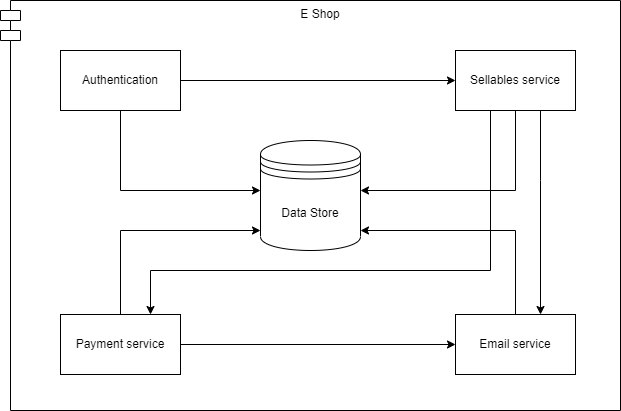
\includegraphics[scale=0.6]{img/komponentu diagrama.drawio.png}
    \caption{E Shop monolito naudojamų komponentų diagrama}
    \label{img:e-shop-komponentai}
\end{figure}


Šiame grafe galima pamatyti, jog „Mono2Micro“ išskyrė 3 mikroservisus (rekomenduotas 3 klasių „mikroservisas“ yra konfigūraciniai failai, kurie priklauso visoms klasėms):
\begin{itemize}
    \item \verb|partition0| -- produktų mikroservisas

    \item \verb|partition1| -- autentikacijos mikroservisas

    \item \verb|partition2| -- pirkimų ir elektroninio pašto mikroservisas
\end{itemize}


Galima pastebėti, jog yra klasių, kurios nebuvo priskirtos jokiam mikroservisui. Tai yra klasės, kurios nebuvo kviečiamos ar kitaip naudojamos panaudos atvejų fiksavimo metu. Pasinaudojus šio grafo informacija, visi Java failai, priklausantys vienam mikroservisui, bus sukelti į naują mikroservisą. Jei failas yra naudojamas ir viename, ir kitame servise, vadinasi jis turi priklausyti abiem servisams. Kitaip sakant, jis bus dubliuojamas. Kiekvienas servisas turės savo duomenų bazę. Kvietimai tarp metodų bus pakeisti į REST protokolo kvietimus. Nauja architektūra, pagal „Mono2Micro“ rekomendaciją, pavaizduota \ref{img:nauja-architektura} pav. 

\begin{figure}[H]
    \centering
    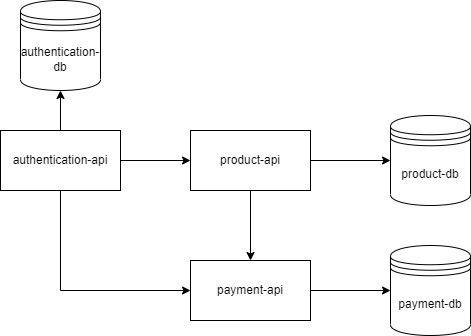
\includegraphics[scale=0.6]{img/microservices-new.png}
    \caption{„Mono2Micro“ rekomenduojama architektūra}
    \label{img:nauja-architektura}
\end{figure}

Kadangi duomenų ryšiai šioje programoje yra paprasti ir lentelės nenaudoja viena kitos duomenų, duomenų migravimas gali būti tiesiog iškeliant duomenis iš vienos lentelės į mikroserviso duomenų bazę. Šio darbo metu duomenų migravimas nebuvo atliktas.

\subsubsection{Ekspertų vertinimas}
Vertinant „Mono2Micro“ buvo pasitelkti trys vyresnieji Java programuotojai, kurie atliko esamos monolitinės programos ir įrankio pasiūlytos mikroservisų architektūros lyginamąją analizę. Jų išvados atskleidė keletą vertų dėmesio „Mono2Micro“ rekomendacijų trūkumų. Visų pirma jie pastebėjo, kad „Mono2Micro“ nesiūlė įtraukti įprastų komponentų, kurie paprastai yra susiję su mikroservisų architektūra, pavyzdžiui, apkrovos balansavimo įrenginio (angl. \emph{Load Balancer}) arba API vartų (angl. \emph{API gateway}). Šie elementai, padedantys valdyti duomenų srautą ir užtikrinti veiksmingą ryšį tarp paslaugų, yra labai svarbūs patikimai ir keičiamo dydžio mikroservisų architektūrai.

Be to, programuotojai pažymėjo, kad „Mono2Micro“ rekomendavo iš monolito išskirti tik vieną „payment-api“ servisą. Tačiau jie nustatė, kad šią paslaugą būtų galima toliau skaidyti į „payment-api“ ir „mail-api“ mikroservisus. Šis pastebėjimas buvo pagrįstas prielaida, kad ateityje „mail-api“ funkcijos greičiausiai išsiplės, todėl bus reikalingas atskiras mikroservisas. Dėl to kyla klausimų dėl priemonės gebėjimo numatyti būsimą įvairių funkcinių sričių augimą ir jos gebėjimo pateikti optimaliai detalizuotas rekomendacijas dėl mikroservisų architektūros.

Šios išvados rodo, kad nors „Mono2Micro“ gali pateikti vertingų rekomendacijų, kaip skaidyti monolitinę programą, ji gali nevisiškai atspindėti visus mikroservisų architektūros niuansus. Tai pabrėžia, kad kartu su tokių priemonių naudojimu reikia žmogiškųjų žinių ir strateginio įžvalgumo, ir pabrėžia nuolatinio „Mono2Micro“ rekomendacijų algoritmų patvirtinimo ir tobulinimo svarbą.

Kadangi įrankis parekomendavo 3 mikroservisus, o ekspertai įžvelgė 4, galima teigti, jog šiuo atveju mikroservisų rekomendacijų tikslumas yra lygus 75 \%. Reikia atsižvelgti, jog vienas šitas eksperimentas nepateikia tikrų „Mono2Micro“ sugebėjimų. Kad ši metrika būtų tikslesnė, privaloma atlikti daugiau tokių bandymų su didesniu skirtingų monolitų kiekiu.

\subsubsection{Sėkmingo vykdymo rodiklis}
Siekiant empiriškai įvertinti „Mono2Micro“ patikimumą, buvo atliktas eksperimentas, kurio metu pakartotinai migruota ta pati monolitinė programa. Pastebėtina, kad visų 50 bandymų metu „Mono2Micro“ sėkmingai generavo rezultatus ir pasiekė 100 \% sėkmingo vykdymo rodiklį. Toks nuoseklus veikimas atliekant pakartotinius bandymus pabrėžia įrankio veikimo patikimumą, nes jis sugebėjo išanalizuoti duotą monolitinę programą ir kiekvieną kartą be jokių klaidų ar problemų pateikti pertvarkymo rekomendacijas.

Nors šis eksperimentas neparodo, ar įrankis visada tiksliai sugeneruoja mikroservisų rekomendacijas, jis parodo, jog net ir varomas dirbtiniu intelektu šis įrankis sugeba sugeneruoti vienodą rezultatą. Eksperimentas parodo, jog įrankis yra deterministinis.

\subsection{Rezultatų pagrįstumas}
Siekdami veiksmingai įvertinti „Mono2Micro“ pagrįstumą, vertinimas buvo vykdomas atsižvelgiant į įgyvendinimo sėkmės rodiklį. Įgyvendinimo sėkmės rodiklis parodo, koks skaičius rekomenduotų mikroservisų, kai jie yra sudiegti, be sutrikimų atlieka numatytas funkcijas ir gal net pagerina bendrą sistemos funkcionalumą, procentinę dalį.

Atliekant vertinimą buvo išbandyti pagrindiniai panaudos atvejai, įskaitant autentifikavimą ir naudotojo kūrimą, produkto elementų kūrimą, paiešką, filtravimą ir pašalinimą ir mokėjimo užbaigimą ir el. pašto siuntimą. Šie bandymai buvo atlikti naudojant „JMeter“ - žinomą programą, sukurtą testuoti programų našumui. Rezultatai parodė, kad naujai sukurtoje mikroservisų architektūroje visi testavimo atvejai sėkmingai atlikti, t.y. grąžino 2xx atsakymo kodą (angl. \emph{response code}). Pažymėtina, kad, palyginus su monolitine sistema, buvo tikėtinas vėlavimo padidėjimas, kuris yra įprastas reiškinys dėl papildomų tinklo apkrovų mikroservisų architektūroje ( žr. pav. \ref{img:latency}). Taigi galima teigti, jog įgyvendinimo sėkmės rodiklis yra 100 \%, nes visi panaudos atvejai vis dar buvo sėkmingai įvykdyti.

\subsection{Įrankio panaudojamumo vertinimas}
Šio įrankio panaudojamumui vertinti nebus naudojami įprasti vertinimo metodai, nes tai bus tik autoriaus nuomonė, kuri gali neatspindėti kitų „Mono2Micro“ naudotojų nuomonės. Kadangi autorius anksčiau nebuvo dirbęs su šiuo įrankiu, vertinimas yra laikomas nešališku. Bus vertinami šie panaudojamumo elementai: terminalo vartotojo sąsaja, interaktyvi aplinka ir dokumentacija. Šitie elementai buvo pasirinkti dėl to, nes jie yra pagrindiniai elementai, norint sėkmingai dirbti su šituo įrankiu. Šių elementų didelis panaudojamumo matas reikštų, jog pats įrankis turi aukštą panaudojamumą. Kiekvienas šių elementų bus vertinamas skalėje 1-5, kur 1 - visiškai nesuprantama vartotojo sąsaja, o 5 - visiškai aiški ir suprantama sąsaja.

\subsubsection{Terminalo vartotojo sąsaja}
Pagrindinės „Mono2Micro“ komandos veikai terminale. kadangi tai yra patys svarbiausi šio įrankio žingsniai, geras terminalo sąsajos panaudojamumas yra itin svarbus. Kiekvienai komandai buvo suteikta pagalbos funkcija \verb| --help|. Ši komanda detaliau aprašo priimtinus komandos argumentus, paaiškina jų reikšmę, nurodo kurie elementai yra būtini, o kurie ne. Komandų nėra daug ir jas galima labai greitai išmokti, o jei pritrūksta kurių nors detalių, kurių nesuteikia pagalbos komanda, galima pasiremti dokumentacija.

Tačiau klaidų atveju, terminalas nesuteikia daug naudingos informacijos, ir nei pagalbos funkcija, nei dokumentacija nenurodo, kaip elgtis nenumatytų klaidų atvejais. Aiškus klaidų nurodymas yra itin svarbus bet kokiam įrankiui, kitaip naudotojas yra priverstas naudotis IBM pagalbos linija, o tai yra daug laiko trunkantis procesas.

Vertinimas -- \textbf{3}.

\subsubsection{Interaktyvi aplinka}
Interaktyvioje aplinkoje galima peržiūrėti rekomenduojamų mikroservisų grafą. Šis grafas labai aiškiai nurodo, kurios klasės gali priklausyti kokiam mikroservisui. Interaktyvioje aplinkoje galima peržiūrėti rekomenduojamus mikroservisus pagal panaudos atvejus, arba pagal natūralių gijų panašumą -- priklausomai nuo naudotojo poreikių. Taip pat yra galimybė sukurti savo mikroservisų rekomendacijas naudojantis esamomis klasėmis. Aplinka yra minimalistinė, nėra nereikalingos informacijos, yra susipažinimo su aplinka funkcija. Išmokti ja naudotis nėra sudėtinga.

Interaktyvi aplinka nesuteikia galimybės išimti klasės iš rekomenduojamų mikroservisų. Didelėse sistemose, klasių gali būti labai daug, ir kai kurių elementų panaikinimas iš darbo lauko labai supaprastina visos architektūros suvokimą. Jei yra poreikis panaikinti tam tikras klases, tai galima atlikti tik redaguojant grafo \verb|.json| failą.

Vertinimas -- \textbf{4}.

\subsubsection{Dokumentacija}
IBM suteikia gan detalią dokumentaciją, kurioje yra aprašyti visi žingsniai, nuo „Mono2Micro“ įsidiegimo, iki sugeneruotų servisų diegimo IBM aplinkoje. Dokumentacija gerai aprašo pagrindines terminalo komandas bei suteikia itin daug informacijos apie interaktyvią aplinką. Dokumentacija yra kupina pavyzdžių, o tai padeda lengviau suprasti vykdomus veiksmus. Taip pat yra pateikiami tikėtini komandų rezultatai, kokie failai turi būti sugeneruoti, bei kokie kiti žingsniai turės būti atlikti vėliau.

Dokumentacijoje nėra aprašoma, kaip reikia elgtis tam tikrų klaidų atveju. Joje nėra informacijos, kokios klaidos yra tikėtinos, kaip jų išvengti. Ši informacija yra kritinė, nes kol yra išmokstama dirbti su „Mono2Micro“, susiduriama su dideliu kiekiu netikėtų klaidų.

Vertinimas -- \textbf{3}.

\subsection{Rezultatai}
Eksperimentų metu pasiekti rezultatai yra pavaizduoti \ref{table:rezultatai} lentelėje. Remdamiesi „Mono2Micro“ vertinimo rezultatais, galima daryti išvadas, kad „Mono2Micro“ pasižymi dideliu našumu ir perspektyviu naudingumu migravimo procese. Rekomendacijų tikslumas siekia 75 \%, o tai rodo, kad nors priemonės pasiūlymai iš esmės atitinka ekspertų nuomonę, yra tokių atvejų, kai žmogiškosios žinios gali suteikti daugiau įžvalgų ar patobulinimų. Tai rodo, kad priemonė yra vertinga pagalba, nors ir nepakeičia ekspertų būtinumo. „Sėkmingo vykdymo rodiklis“ ir „Sėkmingo įgyvendinimo rodiklis“ siekia 100 \%, o tai rodo, kad įrankis geba generuoti rezultatus be klaidų ir kad jo rekomenduojamos mikroservisai sėkmingai veikia. Tai tvirtas „Mono2Micro“ veikimo patikimumo ir rekomendacijų veiksmingumo įrodymas. Apibendrinant galima teigti, jog šis įrankis sugeba kokybiškai atlikti monolitinės programos migravimą.

Įrankio panaudojamumo požiūriu „Mono2Micro“ galima gerinti, ypač terminalo sąsają ir dokumentaciją, kurios abi įvertintos 3 balais iš 5. Šių sričių patobulinimai galėtų pagerinti naudotojo patirtį ir palengvinti su šia priemone susijusį mokymosi procesą. Interaktyvioji aplinka, įvertinta 4 balais iš 5, yra ypač gerai įvertinta, o tai rodo, kad ji yra veiksminga ir patogi naudoti. Atsižvelgiant į šiuos įvertinimus, akivaizdu, kad nors „Mono2Micro“ gerai atlieka savo funkcijas, į naudotojų atsiliepimus reikėtų atsižvelgti nuolat tobulinant jo vartotojo sąsają ir dokumentaciją, skiriant daugiau dėmesio klaidų taisymams ir aprašymams.

\begin{table}[!ht]
    \centering
    \caption{„Mono2Micro“ vertinimo rezultatai}
    \label{table:rezultatai}
    \begin{tabular}{|l|l|}
    \hline
        Mikroservisų rekomendacijų tikslumas & 75 \% \\ \hline
        Sėkmingo vykdymo rodiklis & 100 \% \\ \hline
        Įgyvendinimo sėkmės rodiklis & 100 \% \\ \hline
        \textbf{Vidurkis} & \textbf{91 \%} \\ \hline
        ~ & ~ \\ \hline
        Terminalo vartotojo sąsaja & 3 / 5 \\ \hline
        Interaktyvi aplinka & 4 / 5 \\ \hline
        Dokumentacija & 3 / 5 \\ \hline
        \textbf{Vidurkis} & \textbf{3.3 / 5} \\ \hline
    \end{tabular}
\end{table}

\subsection{Patarimai ir rekomendacijos} % o gal \section{} ?
Naudojantis „Mono2Micro“ viskas buvo remiamasi oficialia šio įrankio dokumentacija. Ji yra viešai prieinama ir aprašo visą procesą, nuo „Mono2Micro“ diegimo iki naujų mikroservisų diegimo IBM aplinkoje. Tačiau dokumentacijoje buvo aprašyti tik laimingo srauto (angl. \emph{happy flow}) scenarijai. Jei naudojimosi įrankiu metu atsiranda klaidos, tai jos dokumentacijoje nėra indikuojamos, o pats klaidų formatas yra labai neinformatyvus - tai įprastai yra tik Python kalbos klaidos pranešimai (angl. \emph{stack trace}). Susisiekti su IBM pagalbos linija taip pat yra itin sudėtinga. Kadangi tai yra tarptautinė įmonė, IBM normalizuoja savo pagalbos linijos procesą, kuris yra ilgai trunkantis ir dažnu atveju skiriamas tik įmonėms, o ne individualiems asmenims.

Darbo metu buvo nustatyti šie bendri pastebėjimai, kurie nėra paminėti dokumentacijoje, tačiau, autoriaus nuomone, jie yra labai svarbūs ir privalo būti paminėti:
\begin{itemize}
    \item \textbf{„Mono2Micro“ nėra suderintas su kompiliavimo metu generuojamu kodu}. Naudojant Java Spring Boot karkasą, labai dažnai yra sutinkamas generuojamas kodas, kuris pagreitina programuotojų darbą išvengiant šabloninio kodo kūrimo. Naudojantis tokiomis bibliotekomis, kaip \emph{Lombok} ar \emph{Map Struct} labai didelė dalis kodo yra sugeneruojama naudojantis anotacijomis arba interfeisais. Vykdant statinę kodo analizę su \verb|mono2micro analyze| komanda, šis sugeneruotas kodas yra nuskaitomas, tačiau naudojantis \verb|mono2micro recommend| komanda, dirbtinio intelekto variklis nesugeba atrasti šio sugeneruoto kodo, ir tai priverčia visą procesą sustoti. Šios problemos sprendimas yra paprastas, bet labai ne praktiškas -- pakeisti sugeneruotą kodą įprastu kodu. Tokiu būdu įrankis nepameta klasių ir metodų informacijos ir gali sėkmingai vykdyti savo užduotis.

    \item \textbf{Kuo daugiau bibliotekų yra naudojama monolite, tuo daugiau bus prigeneruota šiukšlinės informacijos}. Didelėse programose įprastai būna daug konfigūracinių elementų, arba bibliotekų, kurios priklauso nuo kitų bibliotekų. Statinės analizės metu yra sukuriama labai daug informacijos apie visas klases, metodus ir ryšius tarp metodų, taigi visa ne su verslo logika susijusi informacija taip pat patenka į šiuos duomenis. Galų gale vykdant rekomendacijos komandą, susiduriama su panašia problema kaip pirmame šio sąrašo punkte - nesutampa statinės analizės sugeneruotų duomenų ir programos žurnalo (log file) duomenys. Šią problemą galima sutvarkyti statinės analizės komandai nurodžius, kurias bibliotekas (Java paketus) įtraukti į statinę analizę, o kurių ne. Tačiau sprendimas, kurios bibliotekos turi būti įtrauktos nėra lengvai priimamas. Vienintelis būdas yra keisti šiuos parametrus ir bandyti atlikti migravimą toliau tol, kol pasiseks. Jei migravimas yra sėkmingas, „Mono2Micro“ sukuria rekomendacijų grafą su visų įtrauktų ir atrastų bibliotekų klasėmis, o tai yra nereikalinga šiukšlinė informacija.

    \item \textbf{Nėra galimybės redaguoti galutinio rekomendacijų grafo}. „Mono2Micro“ interaktyvi aplinka suteikia galimybę priskirti klases kitiems mikroservisams, tačiau nesuteikia galimybės ištrinti tam tikras klases iš šio grafo. Ši problema siejasi su antru punktu iš šio sąrašo. Jei galutiniame rekomendacijų grafe yra daug šiukšlinės informacijos, tai kenkia bendro vaizdo matymui vartotojui. Jei vartotojas nori panaikinti klases iš grafo, tai jis to negali atlikti interaktyvioje aplinkoje. Tai galima atlikti tik redaguojant grafo \verb|.json| failą. Tačiau kai yra daug klasių ir ryšių, klasių naikinimus reikia atlikti visoms klasėms. Kad šis darbas būtų atliktas, dar yra privaloma suprasti grafo failo struktūrą, kad rankomis redaguojamas grafas vėliau nebūtų sugadintas. Šio darbo autoriaus rekomendacija yra stengtis įtraukti kuo mažiau bibliotekų statinės analizės fazėje (\verb|mono2micro analyze|).

    \item \textbf{Geras monolitinės programos padengimas integraciniais testais pagreitina migravimo laiką}. Dokumentacijoje nėra paminėta, tačiau panaudos atvejų fiksavimą (\verb|mono2micro usecase|) galima atlikti ne tik rankiniu būdu atliekant visus panaudos atvejui būdingus veiksmus, bet ir pasinaudojant egzistuojančiais testais, kurie padengia tą panaudos atvejį. Svarbiausia yra nepamiršti, jog nesvarbu ar panaudos atvejai yra fiksuojami rankiniu būdu, ar pasinaudojant testais, visų metodų įėjimo, išėjimo bei kvietimo informacija privalo būti rašoma į žurnalą pasinaudojant IBM suteiktu dvejetainio instrumentavimo agentu \emph{„Minerva“}, kuris atlieka visų metodų fiksavimą ir užrašo jų kvietimus, kartu su laiko žyma, į žurnalą.

    \item \textbf{Įrankio sugeneruotas mikroservisų kodas nėra visur pritaikomas}. Dokumentacijoje yra minama, jog „Mono2Micro“ yra skirtas IBM Websphere Liberty serveriuose veikiančioms sistemoms, tačiau nepamini, jog sugeneruotas mikroservisų kodas naudoja IBM bibliotekas, kurių negalima atrasti bendroje \emph{„Maven“} repozitorijoje. Taip pat sugeneruotas kodas nėra optimizuotas. Visur, kur tarp mikroservisų yra ryšys tarp dviejų klasių, nesvarbu ar tai serviso ar repozitorijos klasė, yra sugeneruojamas HTTP kvietimo kodas, o tai dažnose vietose yra nelogiška ir neatitinka gerųjų programų projektavimo praktikų.

    \item \textbf{Įrankio sugeneruotas kodas yra nepadengtas testais}. Net jei monolitinė programa turi didelį padengimą testais, sugeneruotas kodas testų nemigruoja, tai yra privaloma visus testus rankiniu būdu perrašyti naujoje architektūroje.
\end{itemize}

\sectionnonum{Rezultatai}
Šio darbo metu pasiekti rezultatai:
\begin{itemize}
    \item Išanalizuota monolitinė sistema „E Shop“: aprašyti esantys moduliai, panaudos atvejai, dydis, padengimo testais dydis, duomenų struktūra ir klasių ryšiai.

    \item Atlikus sistemos analizę, naudojant „Mono2Micro“ įrankį buvo pradėtas „E Shop“ programos migravimas. Procedūra, apimanti visus etapus nuo pradinio planavimo iki sėkmingo užbaigimo, buvo kruopščiai dokumentuojama. Šis įrašas suteikia vertingų įžvalgų ir pakartojamą veiksmų planą būsimiems perkėlimo procesams, taip išplečiant tyrimo poveikį už šios programos ribų.

    \item Buvo atlikti suplanuoti eksperimentai, kuriais siekta įvertinti „Mono2Micro“ kokybę ir naudingumą migruojant monolitinę programą. Testavimo scenarijų įvairovė leido nuodugniai ištirti įrankio galimybes įvairiomis sąlygomis, todėl buvo galima patikimai įvertinti jo funkcionalumą ir patikimą veikimą.

    \item Iš atliktų eksperimentų buvo nustatytos išvados, kurios įrodo „Mono2Micro“ veiksmingumą.

    \item Surinktos ir aprašytos pastabos bei patarimai apie įrankio panaudojamumą būsimiems šio įrankio naudotojams.
    
    
\end{itemize}

\sectionnonum{Išvados}
\begin{itemize}
    \item „Mono2Micro“ veikia su Java kalba parašytomis programomis ir gali monolitinės programos migravimą atlikti su Spring Boot karkasu.

    \item „Mono2Micro“ pademonstravo aukštą patikimumo laipsnį. Įrankis sugeba sugeneruoti mikroservisų rekomendacijas ir tai atlikti be nenumatytų klaidų, tačiau yra privaloma atlikti daug paruošiamųjų darbų.

    \item Nors „Mono2Micro“ pateikia dažnu atveju geras mikroservisų rekomendacijas, vis dar išlieka srities ekspertų reikalingumas, nes šis įrankis dar nesugeba atlikti tokių prognozių, kokias įžvelgia žmogus.

    \item Parekomenduoti ir implementuoti mikroservisai atlieka savo pirmines užduotis ir nėra prarandami panaudos atvejai ar jų dalys. Nors šios užduotys yra atliekamos truputį lėčiau, tai yra įprasta mikroservisų architektūroje.

    \item „Mono2Micro“ turi pakankamai aiškią vartotojo sąsają, tačiau nenumatytų klaidų atveju nepateikia grįžtamojo ryšio, kodėl nutiko klaida ar kaip jos išvengti.

    \item Nors „Mono2Micro“ yra įrankis skirtas mikroservisų architektūros pagrindams suteikti, šis įrankis nepateikia rekomendacijų susijusių su įprastais mikroservisų architektūros aspektais, kaip krūvio skirstytojas, ar pačių duomenų migravimas.

    \item Būsimi „Mono2Micro“ tyrimai turėtų labiau akcentuoti įrankio panaudojamumą atliekant bandymus su didesniu kiekiu skirtingų monolitinių programų.

\end{itemize}

\printbibliography[heading=bibintoc]

\appendix  % Priedai
% % Prieduose gali būti pateikiama pagalbinė, ypač darbo autoriaus savarankiškai
% % parengta, medžiaga. Savarankiški priedai gali būti pateikiami ir
% % kompaktiniame diske. Priedai taip pat numeruojami ir vadinami. Darbo tekstas
% % su priedais susiejamas nuorodomis.

% \section{Neuroninio tinklo struktūra}
% \begin{figure}[H]
%     \centering
%     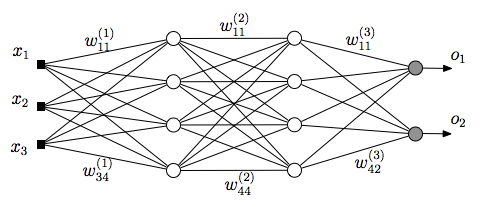
\includegraphics[scale=0.5]{img/MLP}
%     \caption{Paveikslėlio pavyzdys}
%     \label{img:mlp}
% \end{figure}

\section{Sugeneruotas mikroservisų rekomendacijų grafas}
\begin{figure}[H]
    \centering
    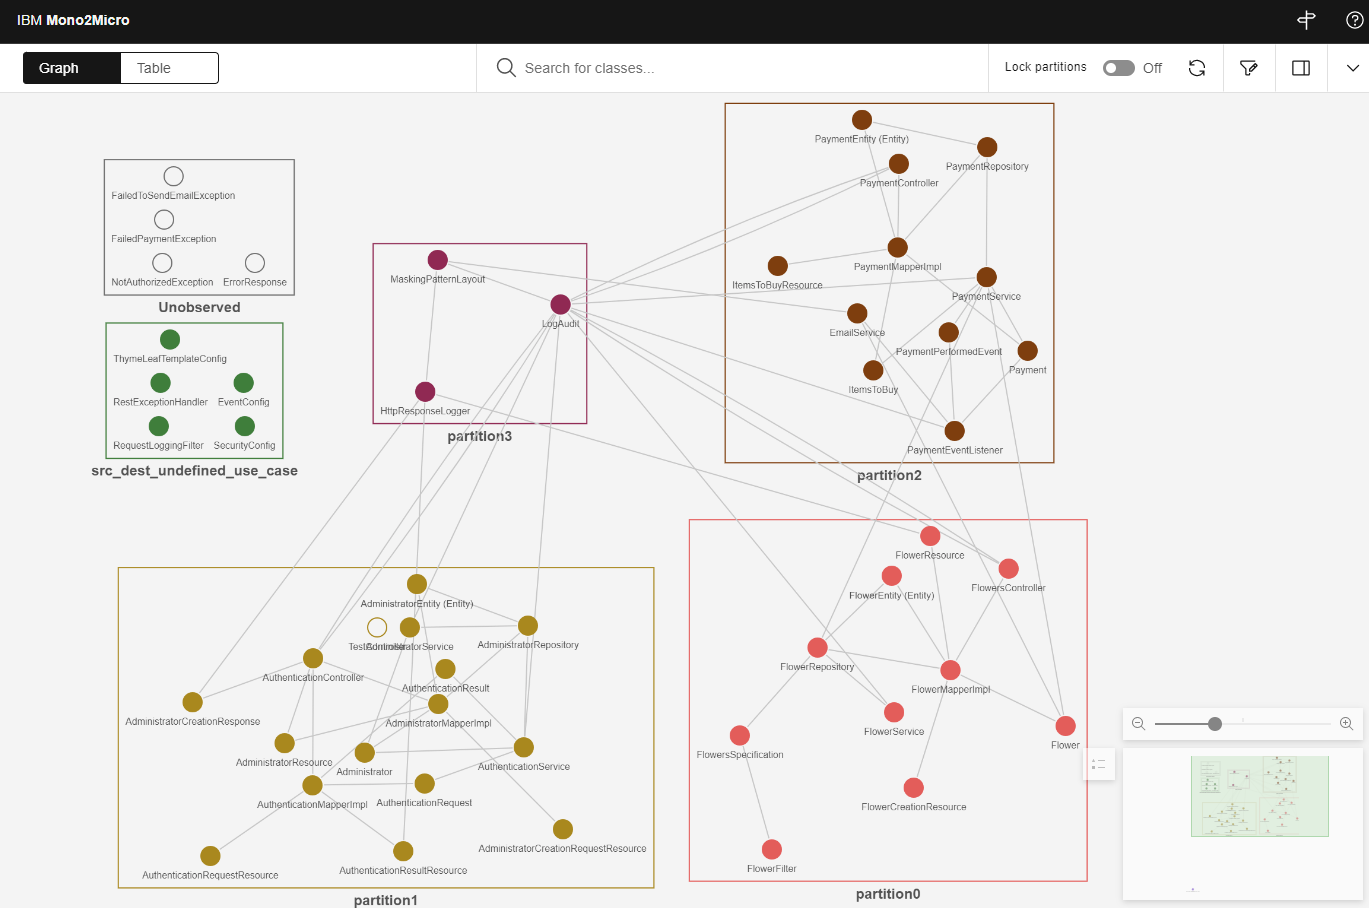
\includegraphics[scale=0.4]{img/grafas.png}
    \caption{Sugeneruotas grafas su mikroservisų rekomendacijomis}
    \label{img:grafas}
\end{figure}

\section{Monolitinės ir mikroservisų architektūros HTTP kvietimų srautų palyginimas}
\begin{figure}[H]
    \centering
    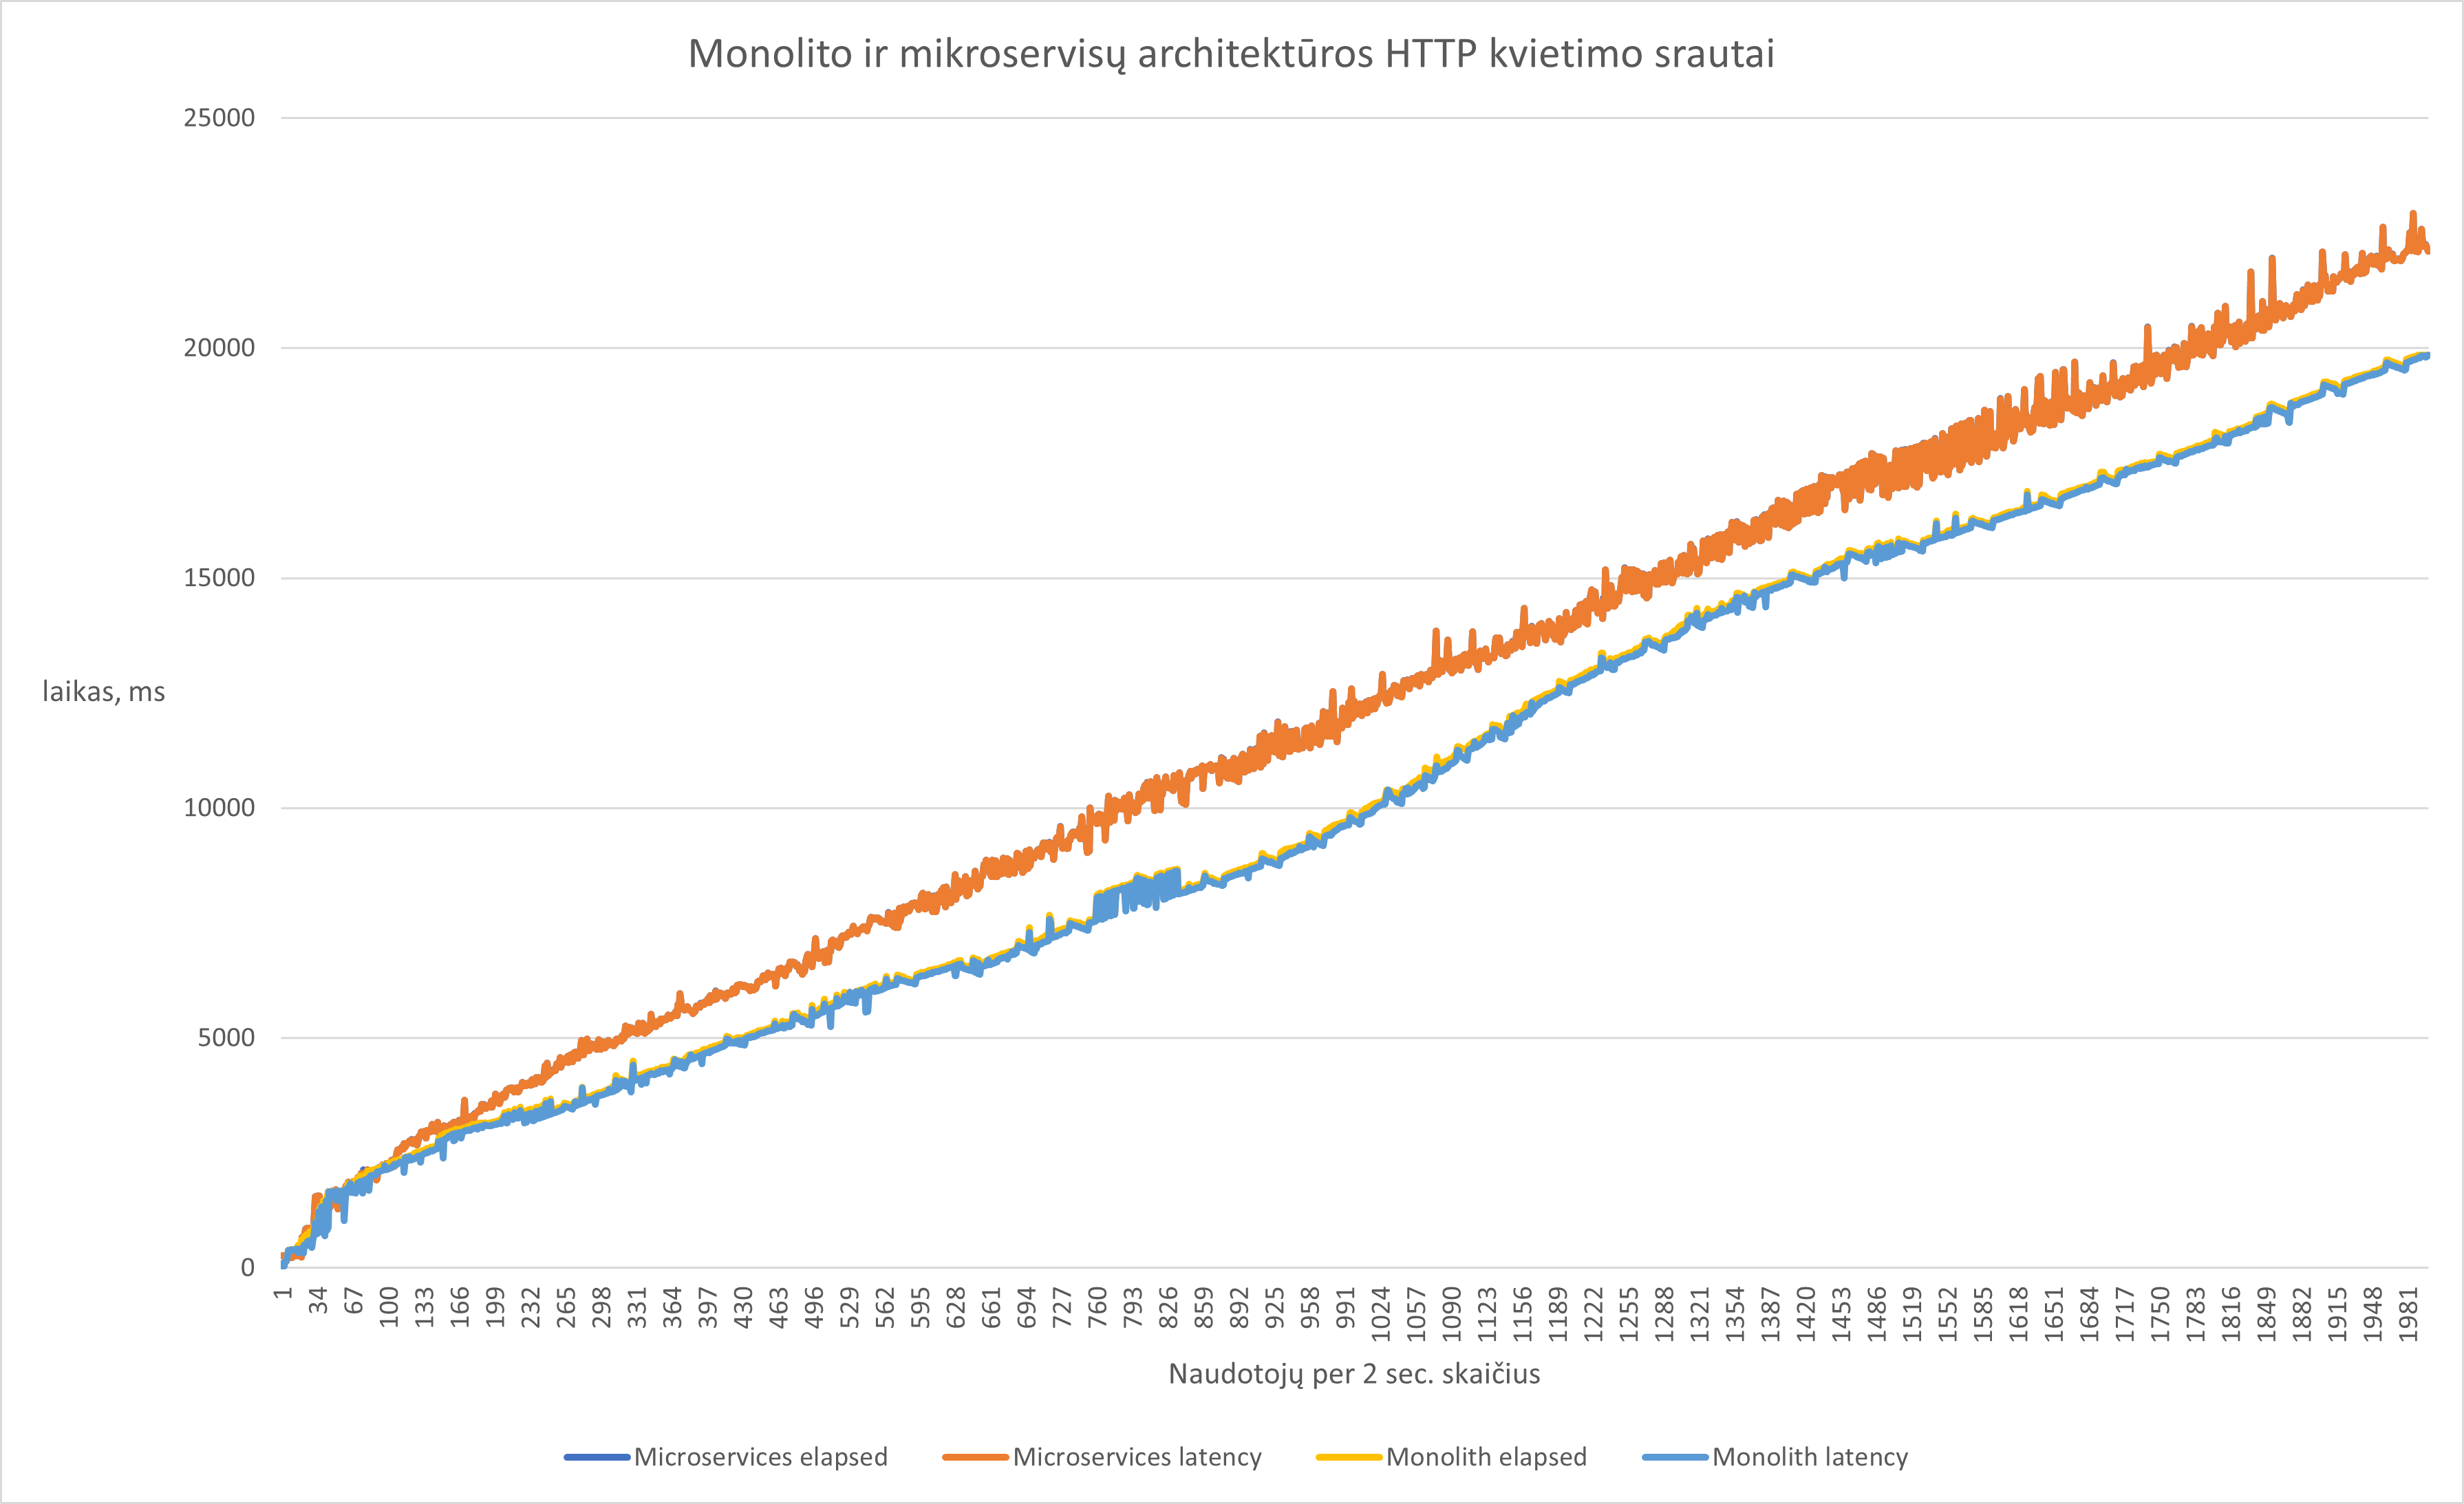
\includegraphics[scale=0.6]{img/latency.png}
    \caption{Monolitinės ir mikroservisų architektūros HTTP kvietimų srautų palyginimas}
    \label{img:latency}
\end{figure}

\end{document}
